\documentclass{article}

% The ICLR 2027 workshop template is not yet public.  We use the latest
% official ICLR style verbatim and keep the year-specific dependency isolated.
\usepackage{iclr2026/iclr2026_conference,times}

\input{iclr2026/math_commands.tex}
\usepackage{amsmath,amssymb,bm}
\usepackage{booktabs}
\usepackage{graphicx}
\usepackage{multirow}
\usepackage{array}
\usepackage{float}
\usepackage{xcolor}
\usepackage{hyperref}
\usepackage{url}
\usepackage{microtype}

\graphicspath{{figures/}}

\newcommand{\method}{\textsc{MadNLP4NN}}
\newcommand{\kkt}{\mathrm{KKT}}
\newcommand{\dlpack}{\textsc{DLPack}}
\newcommand{\lbfgs}{\textsc{L-BFGS}}
\newcommand{\gn}{\textsc{Gauss--Newton}}
\newcommand{\cpu}{\textsc{CPU}}
\newcommand{\gpu}{\textsc{GPU}}
\newcommand{\success}{\textsc{Success}}
\newcommand{\dataset}{\mathcal{D}}
\newcommand{\norminf}[1]{\lVert #1\rVert_{\infty}}
\newcommand{\normtwo}[1]{\lVert #1\rVert_{2}}
% Auto-generated by experiments/analysis/build_iclr_artifacts.py.
\newcommand{\PFRCaseOneSparseCPU}{43.3}
\newcommand{\PFRCaseOneDenseCPU}{0.59}
\newcommand{\PFRCaseThreeGPU}{2.27}
\newcommand{\PFRCaseThreeGPULo}{2.25}
\newcommand{\PFRCaseThreeGPUHi}{2.32}
\newcommand{\PFRCaseThreeCPU}{19.71}
\newcommand{\PFRCaseThreeCPULo}{19.71}
\newcommand{\PFRCaseThreeCPUHi}{19.91}
\newcommand{\PFRCaseThreeSpeedup}{8.7}
\newcommand{\PFRCaseThreeIpopt}{27.84}
\newcommand{\PFRCaseThreeLBFGS}{530.36}
\newcommand{\DarcyRouteBase}{115}
\newcommand{\DarcyRouteTotal}{120}
\newcommand{\DarcyRouteOverhead}{7.7}
\newcommand{\ReplayGroups}{120}
\newcommand{\ReplayAgreement}{35}
\newcommand{\ReplaySolves}{360}
\newcommand{\ReplayOutfitsTruth}{352}
\newcommand{\ReplayGNFNOWinsThirtyTwo}{59}
\newcommand{\ReplayExactPDEWinsThirtyTwo}{13}
\newcommand{\ReplayGNPDEWinsThirtyTwo}{22}
\newcommand{\ReplayLBFGSPDEWinsThirtyTwo}{25}
\newcommand{\ReplayPairedFNOReduction}{0.095}
\newcommand{\ReplayPairedFNOReductionLow}{0.065}
\newcommand{\ReplayPairedFNOReductionHigh}{0.133}
\newcommand{\ReplayPairedFNOPValue}{0.00049}
\newcommand{\ReplayPairedPDEDelta}{1.20}
\newcommand{\ReplayPairedPDEDeltaLow}{-1.10}
\newcommand{\ReplayPairedPDEDeltaHigh}{2.96}
\newcommand{\ReplayPairedPDEPValue}{0.266}
\newcommand{\ReplayGNTime}{0.714}
\newcommand{\ReplayGNSurrogate}{0.37}
\newcommand{\ReplayGNPDE}{5.09}
\newcommand{\ReplayLBFGSTime}{1.43}
\newcommand{\ReplayLBFGSSurrogate}{0.49}
\newcommand{\ReplayLBFGSPDE}{4.13}
\newcommand{\ReplayExactTime}{1.95}
\newcommand{\ReplayExactSurrogate}{0.76}
\newcommand{\ReplayExactPDE}{4.68}
\newcommand{\MNISTStarts}{5}
\newcommand{\MNISTSolved}{15}
\newcommand{\MNISTTotal}{15}
\newcommand{\MNISTExactMedianObjective}{4.736}
\newcommand{\MNISTLBFGSMedianObjective}{5.590}
\newcommand{\DarcyExactMemory}{33.54}
\newcommand{\DarcyLBFGSMemory}{0.99}

% Generated by experiments/analysis/analyze_sequence_and_topology.py
\newcommand{\PFRSequenceSuccesses}{1100}
\newcommand{\PFRSequenceTotal}{1100}
\newcommand{\PFRWarmCPUColdIter}{10}
\newcommand{\PFRWarmCPUPrimalIter}{6}
\newcommand{\PFRWarmCPUBarrierIter}{3}
\newcommand{\PFRWarmGPUColdIter}{10}
\newcommand{\PFRWarmGPUPrimalIter}{4}
\newcommand{\PFRWarmGPUBarrierIter}{3}
\newcommand{\PFRWarmEqualBarrierSteps}{66}
\newcommand{\PFRWarmCPUBarrierTime}{17.1}
\newcommand{\PFRWarmGPUBarrierTime}{32.9}
\newcommand{\PFRPersistentMedianTime}{22.3}
\newcommand{\PFRPersistentMaxTime}{3.00}
\newcommand{\PFRWarmBarrierControlError}{2.48\times 10^{-5}}
\newcommand{\FNOShapeMinMemory}{32.72}
\newcommand{\FNOShapeMaxMemory}{37.25}
\newcommand{\FNOShapeMemoryDelta}{4.52}
\newcommand{\FNOShapeMemoryIncrease}{13.8}
\newcommand{\FNOShapeMaxParameterMismatch}{1.0}
\newcommand{\FNOShapeTrainedMemory}{32.77}
\newcommand{\FNOShapeRandomMemory}{32.77}
\newcommand{\FNOShapeFastHessian}{65}
\newcommand{\FNOShapeSlowHessian}{132}
\newcommand{\FNOShapeCrossHardwareDelta}{0.22}
\newcommand{\PFRStrictCPUPrimalIter}{6}
\newcommand{\PFRStrictCPUBarrierIter}{4}
\newcommand{\PFRStrictGPUPrimalIter}{4}
\newcommand{\PFRStrictGPUBarrierIter}{4}


\title{Structure Before Hardware: A Regime Map for Optimization with Neural Surrogates}

\author{Anonymous authors}

\begin{document}
\maketitle
\lhead{Under review for an ICLR workshop}

\begin{abstract}
Optimizing through a fixed neural surrogate couples two computational systems:
automatic differentiation through a network and a constrained nonlinear
programming solver.  Moving the first to a GPU does not imply that the
Karush--Kuhn--Tucker (KKT) system should follow, nor that exact curvature is the
right model.  We present \method, an audited JAX--MadNLP interface that exposes
neural derivatives through DLPack device buffers while preserving
problem-supplied Jacobian and Lagrangian-Hessian sparsity.  We isolate four
choices---structure disclosure, curvature, transfer semantics, and KKT
placement---on controlled problems and three established neural-embedded NLP
families.  Correct sparsity reduces a published neural NMPC solve from
\PFRCaseOneDenseCPU\,s to \PFRCaseOneSparseCPU\,ms and reverses the CPU/GPU
ranking; at 7,500 neural equalities, however, GPU KKT is
\PFRCaseThreeSpeedup$\times$ faster than CPU KKT.  A prospectively evaluated
curvature route raises Darcy inversion success from \DarcyRouteBase/\DarcyRouteTotal{}
to \DarcyRouteTotal/\DarcyRouteTotal{} at \DarcyRouteOverhead\% additional warm
time.  At a fixed FNO parameter budget of 1.18M, changing depth and width moves the
exact-Hessian peak from \FNOShapeMinMemory{} to \FNOShapeMaxMemory{} GiB;
parameter count alone does not predict second-order AD memory.  Finally,
independent PDE replay shows that surrogate improvement need
not transfer: Gauss--Newton lowers FNO residual relative to L-BFGS on all
twelve physical instances, while the paired PDE change has a 95\% bootstrap
interval spanning $\ReplayPairedPDEDeltaLow$ to
$\ReplayPairedPDEDeltaHigh$ percentage points.  Descriptive start-level
rankings agree in only \ReplayAgreement/\ReplayGroups{} matched groups.  The
result is a reproducible regime map rather than a single GPU speedup: solver
convergence, systems speed, and application validity remain distinct
requirements.
\end{abstract}

\section{Introduction}
\label{sec:introduction}

Neural networks are increasingly used as differentiable surrogates for
simulators that are too expensive to place directly inside design, estimation,
and control loops.  Once trained, a surrogate is often treated as an ordinary
smooth mapping and embedded in a nonlinear program (NLP).  This pattern appears
in process design, security-constrained power flow, adversarial verification,
and neural-operator inversion
\citep{yang2021modeling,kilwein2023feasibility,bugosen2023flowsheet,li2021fno}.
Modern automatic differentiation (AD) evaluates network
oracles efficiently, while mature primal--dual methods enforce nonlinear
constraints and report stationarity, feasibility, and complementarity
residuals.

The computational consequence is less clear.  A neural-surrogate NLP joins a
deep-learning runtime to a sparse optimization runtime.  Its wall time depends
on at least four coupled choices: (i) which derivative sparsity is disclosed to
the solver; (ii) whether curvature is exact, Gauss--Newton, or quasi-Newton;
(iii) whether framework boundaries stage tensors through host memory; and
(iv) whether the KKT system is assembled and factorized on the CPU or GPU.
Calling the network on a GPU resolves none of the other three choices.

Recent work has established full-space, reduced-space, and gray-box
formulations for neural predictors \citep{ceccon2022omlt,dowson2025mathoptai,
parker2024formulations}.  Most closely, \citet{parker2025gpu} move PyTorch
network derivatives to an A100 while Ipopt and its linear algebra remain on the
CPU.  In parallel, MadNLP and ExaModels demonstrate GPU-resident condensed KKT
methods for large algebraic NLPs
\citep{shin2024opf,pacaud2024dynamic,pacaud2024condensed}.  Together these
results motivate connecting a neural AD runtime to a GPU NLP solver.  Yet an end-to-end
implementation alone would answer only whether this is possible, not when it
is useful.  Small KKT systems cannot amortize GPU setup; a dense derivative
declaration can manufacture an artificial GPU crossover; and avoiding Hessian
callbacks can increase the number of expensive factorizations by an order of
magnitude.

Speed is not the only failure mode.  A KKT point is certified for
the \emph{surrogate} NLP, not for the physical system.  Optimizing a learned
model changes its input distribution and can amplify small prediction errors,
a central concern in offline model-based optimization
\citep{trabucco2021coms,trabucco2022designbench}.  For an inverse problem, a
method that achieves a lower surrogate residual can therefore produce a worse
simulator residual.  Systems benchmarks that omit independent replay can rank
methods precisely while ranking the wrong quantity.

This paper asks four questions:

\begin{enumerate}
  \item When does GPU-resident KKT linear algebra improve time to a
  solver-independent KKT target beyond GPU-accelerated neural AD alone?
  \item Can transfer removal matter after derivative sparsity and cold
  specialization are accounted for?
  \item How do exact, Gauss--Newton, and limited-memory curvature trade time,
  robustness, memory, and local solution quality, and does network topology
  matter after parameter count is fixed?
  \item Do rankings under the optimized surrogate agree with rankings after
  independent simulator replay?
\end{enumerate}

We answer these questions with \method, a JAX--MadNLP interface and an
experiment protocol constructed to vary neural parameter count, decision
dimension, and constraint/output dimension separately.  Our evidence combines
a planted smooth family, the public adversarial-MNIST problem used by the
closest GPU study, all three released neural-surrogate PFR-NMPC cases of
\citet{elorza2025nmpc}, and elliptic Darcy inversion with both a public FNO
split and a fully replayable finite-difference split.

Our contributions are:

\begin{itemize}
  \item \textbf{An audited end-to-end interface.}  DLPack shares CUDA buffers
  between CUDA.jl and JAX, derivative values are copied device-to-device into
  solver-owned storage, and evaluators declare sparse Jacobian and
  Lagrangian-Hessian coordinates.  Pointer identity, mutation, array layout,
  forward parity, and directional derivatives are separately tested.

  \item \textbf{A deployment regime map.}  We separate neural AD placement,
  host staging, KKT placement, curvature, sequence initialization, and cold
  specialization.  Across three published NMPC scales, correct sparsity first
  favors CPU KKT and a larger case then favors GPU KKT by
  \PFRCaseThreeSpeedup$\times$; both conclusions
  disappear in a one-dimensional ``GPU versus CPU'' label.

  \item \textbf{Failure-aware curvature evidence.}  A policy fixed on pilot
  cases runs L-BFGS first and invokes exact curvature only after a common-KKT
  failure.  On disjoint Darcy instances it obtains
  \DarcyRouteTotal/\DarcyRouteTotal{} successes with
  \DarcyRouteOverhead\% overhead over L-BFGS alone.  Other tasks show why this
  is a route rather than a universal L-BFGS recommendation.

  \item \textbf{Optimization-aware validity checks.}  Held-out targets,
  shared multi-starts, representability floors, raw residual audits,
  mechanistic closed-loop replay, and sparse PDE replay are part of the
  benchmark definition.  Failed runs and correctness-based exclusions remain
  documented in the supplementary material.  The
  replay study reveals that surrogate and simulator method rankings agree only
  \ReplayAgreement/\ReplayGroups{} times.
\end{itemize}

We make no new-formulation claim.  The empirical ordering is \emph{structure
before curvature, curvature before hardware, and simulator validation before
application claims}.  It turns an implementation
choice into a falsifiable experimental protocol and identifies which
accelerator regime is actually being measured.

\section{Related Work}
\label{sec:related}

\paragraph{Neural predictors inside mathematical programs.}
Smooth neural networks may be exposed layer by layer (full space), composed
into algebraic expressions (reduced space), or treated as external vector
oracles (gray box).  OMLT automates predictor formulations in Pyomo
\citep{ceccon2022omlt}; \citet{yang2021modeling} analyze embedded,
mixed-integer, and complementarity representations; and
\citet{kilwein2023feasibility} apply smooth neural feasibility surrogates to
security-constrained optimal power flow.  MathOptAI provides full-, reduced-,
and gray-box representations across Julia and PyTorch models
\citep{dowson2025mathoptai}.  The systematic study of
\citet{parker2024formulations} scales these representations to networks with
hundreds of millions of parameters and identifies neural derivative evaluation
as the gray-box bottleneck.  \citet{parker2025gpu} accelerate that bottleneck
with PyTorch on an A100 while retaining CPU Ipopt.  We use their released MNIST
recipe directly and extend the setting to KKT placement, cross-framework
device transfer, problem-supplied sparsity, and their interaction with
curvature.

Published process-optimization studies reinforce that formulation size is not
the only concern.  Neural surrogates can improve speed while changing
convergence reliability and solution error \citep{bugosen2023flowsheet}.
\citet{elorza2025nmpc} compare explicit and external-function embeddings for
three PDE-surrogate NMPC cases and find that replacing mechanistic equations
does not automatically accelerate local NLP solves.  We translate all three
released checkpoints, retain their horizons and objectives, and use the
mechanistic trajectory for an independent closed-loop check.

\paragraph{Nonlinear programming on GPUs.}
Interior-point methods repeatedly assemble and solve sparse KKT systems
\citep{wachter2006ipopt,nocedal2006numerical}.  GPU factorization is difficult
for indefinite systems requiring pivoting.  Condensed and hybrid
reformulations enable pivoting-free or static-pivot GPU factorizations and have
produced substantial gains on optimal-power-flow and dynamic-optimization
instances \citep{shin2024opf,pacaud2024dynamic,pacaud2024condensed}.  Those
studies use GPU-native algebraic modelers; our neural oracle resides in JAX and
crosses a language/runtime boundary.  DLPack provides the common in-memory
tensor representation used by our bridge \citep{dlpack}.  Concurrently,
jaxipm targets a different regime---throughput over batches of same-family NLPs
rather than latency for one large or receding-horizon problem
\citep{viljoen2026jaxipm}.  We therefore do not compare its batched throughput
with our single-instance timings.

Warm-start evaluation depends on which interior-point state is supplied:
\citet{suri2026warp} show that a strong AC-OPF primal point can be a weak
barrier start.  We therefore separate primal, equality-dual, barrier, and
persistent state rather than label all sequence reuse as ``warm start.''

\paragraph{Curvature and benchmarking.}
Exact Lagrangian Hessians can reduce iterations but have quadratic output size
in the decision dimension and potentially much larger AD workspaces.
L-BFGS trades curvature information for a compact history
\citep{liu1989lbfgs}; Gauss--Newton is natural for least-squares inverse
problems \citep{nocedal2006numerical}.  We report KKT success, iterations,
time, and peak memory together, following the
benchmarking principle that failures and common termination tests must remain
visible \citep{dolan2002profiles}.

\paragraph{Inverse design and optimization shift.}
Neural operators learn maps between function spaces and can accelerate
many-query PDE workloads \citep{li2021fno,kovachki2023neuraloperator}.
Gradient-based input optimization through a learned forward model is also the
basis of the neural-adjoint approach \citep{ren2020neuraladjoint}.  However,
offline model-based optimization shows that directly optimizing a learned
objective can exploit errors away from the training distribution
\citep{trabucco2021coms,trabucco2022designbench}.  Classical surrogate model
management similarly restricts or corrects models using high-fidelity
evaluations \citep{alexandrov2000modelmanagement}.  We do not propose a new
offline-MBO algorithm.  We apply the same evaluation requirement to
constrained neural-surrogate NLPs: a solver comparison is incomplete until
surrogate-optimal candidates are evaluated by an independent oracle whenever
one exists.

\section{Problem Setting and Method}
\label{sec:method}

\subsection{A neural-surrogate NLP has three independent scales}

Let $N_{\theta}:\R^{n_N}\rightarrow\R^{q}$ be a fixed, twice
differentiable neural predictor with $p$ trained parameters.  We consider
problems of the form
\begin{equation}
\begin{aligned}
\min_{x\in\R^n}\quad & f(x,N_\theta(s(x))) \\
\text{s.t.}\quad & c(x,N_\theta(s(x)))=0, \\
& d(x,N_\theta(s(x)))\leq 0,\qquad \ell\leq x\leq u,
\end{aligned}
\label{eq:nlp}
\end{equation}
where $s$ selects or transforms the network inputs.  The relevant scales are
not interchangeable: $p$ controls neural work; $n$ controls explicit gradient
and Hessian size; and the number and structure of constraints, denoted $m$,
controls Jacobian and KKT work.  A large-$p$, small-$n$ classifier stresses AD
differently from a moderate-$p$, large-$n$ neural operator or a long-horizon
NLP with many repeated network equalities.

A full-space formulation introduces hidden activations as variables and layer
equations as constraints.  We instead use a gray-box reduced formulation:
MadNLP sees $x$, final network outputs where required, and callable derivatives,
but not hidden activations.  This preserves the network runtime's fused kernels
without declaring the resulting NLP structurally dense.

At each primal--dual iteration, an interior-point method solves a regularized
KKT system schematically written as
\begin{equation}
\begin{bmatrix}
W_k + D_k & J_k^\top \\
J_k       & -R_k
\end{bmatrix}
\begin{bmatrix}\Delta x\\\Delta\lambda\end{bmatrix}
=-r_k,
\qquad
W_k=\nabla_{xx}^2\mathcal{L}(x_k,\lambda_k),
\label{eq:kkt}
\end{equation}
with constraint Jacobian $J_k$.  For interpretation, we decompose a warm solve
into oracle, transfer, KKT, and globalization time.  This is bookkeeping, not
an additive counterfactual: curvature changes the iteration count, while KKT
placement also changes initialization and numerical trajectories.

\subsection{A structure contract between ML and NLP runtimes}

Each evaluator supplies objective, gradient, constraint, Jacobian-vector,
transpose-Jacobian-vector, and Lagrangian-Hessian callbacks.  It may
also declare coordinate patterns $(\mathcal{I}_J,\mathcal{J}_J)$ and lower
triangular $(\mathcal{I}_H,\mathcal{J}_H)$.  Values are gathered from the same
JAX functions used by dense audits.  Thus a sparsity ablation changes only the
information disclosed to the solver, not the mathematical objective,
constraints, precision, start, or derivative engine.

This distinction is material for repeated dynamics.  In PFR case~1, each
network equality at time $t$ depends only on $(x_t,u_t,x_{t+1})$.  The true
Jacobian has 5,200 nonzeros rather than $400\times430=172{,}000$ entries, and
the lower Hessian has 3,049 rather than 92,665 entries.  Cases~2 and~3 use
batched local CNN Jacobians and Hessians that are scattered into global sparse
coordinates; no global $m\times n$ or $n\times n$ dense array is formed.

\subsection{Three placement paths and an audited device boundary}
\label{sec:placement}

All primary paths evaluate the same float64 JAX oracle \citep{jax2018} on the H100:

\begin{description}
  \item[GPU AD $\rightarrow$ CPU KKT.] JAX evaluates network derivatives on
  the GPU, values are materialized on the host, and MadNLP/MUMPS factorizes the
  sparse KKT system on the CPU.

  \item[Host-staged GPU KKT.] MadNLP and cuDSS use GPU arrays, but callback
  values travel through host NumPy storage before returning to the device.
  This is a transfer control: it represents a nominally GPU solver without a
  device-native framework boundary.

  \item[DLPack GPU KKT.] Solver primal and multiplier buffers are imported into
  JAX through DLPack without copying.  JAX results are copied
  device-to-device into solver-owned coordinate buffers.  We do not call this
  entire operation ``zero-copy'': ownership-safe output placement still
  requires a device copy.  Pointer identity, bidirectional mutation, and
  32-MiB transfer latency are tested independently of an NLP solve.
\end{description}

\subsection{Curvature models}

The exact path supplies
\begin{equation}
W(x,\lambda;\sigma)=
\sigma\nabla^2 f(x)+\sum_{i=1}^{m}\lambda_i\nabla^2 c_i(x).
\label{eq:exacthessian}
\end{equation}
For least-squares Darcy objectives
$\frac{1}{2}\|r(x)\|_2^2+\frac{\rho}{2}\|x-x_0\|_2^2$, the
Gauss--Newton model is
\begin{equation}
W_{\mathrm{GN}}(x)=J_r(x)^\top J_r(x)+\rho I.
\label{eq:gn}
\end{equation}
Our implementation explicitly forms its lower-triangular coordinates.  It can
reduce derivative time and iterations relative to L-BFGS, but still has an
$O(n^2)$ output and, as the memory experiment shows, does not remove the AD
workspace bottleneck.

The third path is MadNLP's compact L-BFGS with history 20
\citep{liu1989lbfgs}.  It removes Hessian callbacks but not KKT solves.  A
history sensitivity study (6, 20, 50) is reported in
Appendix~\ref{app:curvature}.  GPU compact L-BFGS is unsupported on the tested
MadNLP/MadNLPGPU stack and is not replaced by a different algorithm.

\subsection{Failure-aware routing and common success}

The paper evaluates one adaptive policy:

\begin{enumerate}
  \item solve from the prespecified start using compact L-BFGS and CPU KKT;
  \item audit finite values, primal/dual residuals, complementarity, bounds,
  and raw application constraints against a common threshold;
  \item if the audit fails, restart from the \emph{same} initial point using
  exact DLPack curvature and GPU KKT.
\end{enumerate}

The rule was selected on three public-Darcy pilot instances and frozen before
evaluation on twelve disjoint instances.  It is a reliability policy, not a
claim that solver status predicts physical validity.  The latter is assessed
separately using coefficient truth, a representability floor, a mechanistic
closed loop, or a sparse PDE solve depending on the benchmark.

\section{Experimental Protocol}
\label{sec:protocol}

\subsection{Benchmarks span different bottlenecks}

Table~\ref{tab:benchmarks} summarizes the benchmark suite.  The controlled
family is used only for mechanism isolation.  The three application families
come from public problem definitions or reproduce the closest prior work.

\begin{table}[t]
\centering
\caption{Benchmark regimes.  $p$ is the number of fixed network
parameters; $n,m$ are NLP variables and general constraints.  $\operatorname{nnz}J$
and $\operatorname{nnz}H$ use the declared coordinate structures.}
\label{tab:benchmarks}
\small
\setlength{\tabcolsep}{3.1pt}
\begin{tabular}{lrrrrr}
\toprule
Problem & $p$ & $n$ & $m$ & $\operatorname{nnz}J$ & $\operatorname{nnz}H$\\
\midrule
Controlled MLP & 0.04--1.20M & 64--784 & 1 & 64--784 & 2K--308K\\
MNIST attack & 0.17--5.01M & 2,362 & 805 & 10,213 & 307,720\\
Darcy/FNO & 1.19M & 256/1,024 & 0 & 0 & 32,896/524,800\\
PFR case 1 & 3.6K & 430 & 400 & 5,200 & 3,049\\
PFR case 2 & 7.5K & 860 & 800 & 20,000 & 11,738\\
PFR case 3 & 0.34M & 7,780 & 7,500 & 1,905,000 & 963,840\\
\bottomrule
\end{tabular}
\end{table}

\paragraph{Tasks.}
The planted tanh-MLP family isolates systems costs at a common KKT point.
MNIST reproduces the public seed, smooth architecture, sample mapping, and
$\ell_1$ target-class problem of \citet{parker2025gpu,lecun1998mnist} at three
network sizes and five starts.  PFR preserves the horizons, bounds, objectives,
initial states, and released MLP/CNN checkpoints
of~\mbox{\citet{elorza2025nmpc}}; case~1 additionally runs a 100-step
mechanistic closed loop.  Float64 JAX/PyTorch discrepancies are below $9.3\times10^{-16}$.

Public Darcy uses the deterministic $64\times64$ NeuralOperator split
\citep{li2021fno,kovachki2023neuraloperator}, twelve prospective instances,
latent $16^2$/$32^2$ fields, and five starts.  Because its historical
preprocessing cannot be replayed without fitting undocumented metadata, PDE
residuals use a separate prespecified 5,000/1,000 split from
\begin{equation}
-\nabla\!\cdot\!\left(e^{a(s)}\nabla u(s)\right)=1,
\qquad u|_{\partial\Omega}=0,
\label{eq:darcy}
\end{equation}
and a specified sparse finite-difference solver.  Its FNO has 1.32\% mean test
error and stored truth replays to $3\times10^{-8}$ relative error.  Three pilot
and twelve disjoint prospective instances use the same two resolutions and
five starts.  Appendix~\ref{app:formulations} gives every mathematical
formulation and data split.

\subsection{Baselines, timing, and statistics}

MadNLP exact CPU, host-staged GPU, DLPack GPU, and compact L-BFGS paths use the
same JAX oracle.  cyipopt/Ipopt supplies an independent solver baseline with
the same coordinate derivatives; OMLT+Ipopt supplies a full-space formulation
baseline on PFR; and SLSQP appears only in a corrected low-dimensional
box-constrained verification case.  We do not compare against penalty Adam: it
changes the constraints and termination definition.  We also make no
JAX-versus-PyTorch speed claim; PyTorch is used for checkpoint parity.

Warm times exclude one preceding cold solve.  GPU work is synchronized.  Short
controlled runs use ten repetitions; PFR cases 1/2/3 use five/five/five warm
runs for the primary MadNLP paths where practical.  Instance/start sweeps use
their sample distributions as repetitions and report medians and interquartile
ranges.  A method succeeds only if it is finite and passes the common primal,
dual, complementarity, bound, and raw application residual threshold.  The
default threshold is $10^{-6}$; MNIST uses $10^{-7}$ solver KKT and $10^{-6}$
raw feasibility.  Local objectives are compared only among successful solves.
For replay-Darcy uncertainty, the sampling unit is one physical instance:
starts are first aggregated within instance and paired method differences use
a fixed-seed nonparametric bootstrap over the twelve instances.  Start-level
winner counts are descriptive and are not treated as 120 independent samples.

A fixed replay makes every initialization policy see the same 100 PFR NLPs;
we vary shifted primal, equality-dual, barrier, and persistent state separately.
A second ablation holds the latent/full resolutions, Fourier modes, precision,
Hessian construction, and roughly 1.18M FNO parameters fixed while changing
depth and width.  Appendix Tables~\ref{tab:warm-start} and
\ref{tab:topology-memory} specify both designs and their exclusions.

All measurements use a single compute server with an NVIDIA H100 80GB GPU and
two Intel Xeon Platinum 8562Y+ sockets (64 physical cores total).
CPU affinity and BLAS/OpenMP thread counts are fixed.  Peak memory is sampled
from the complete process tree and matching GPU PIDs every 20--50\,ms with JAX
preallocation disabled.  Appendix~\ref{app:repro} lists exact software versions
and dataset/model checksums.

\section{Results}
\label{sec:results}

\subsection{Placement has a crossover, not a winner}
\label{sec:placement-results}

The controlled family first isolates decision dimension.  At $n=64$,
exact GPU-AD/CPU-KKT takes 22.6\,ms versus 43.1\,ms for DLPack GPU KKT.  At
$n=784$, the ordering reverses: DLPack takes 95.2\,ms, host-staged GPU KKT
136.1\,ms, and CPU KKT 198.8\,ms.  DLPack wraps a 32-MiB JAX buffer in about
40\,$\mu$s, compared with 10.9\,ms for a staged transfer.  Removing transfer
is measurable, but at small $n$ it cannot amortize solver initialization.

The established PFR family produces the same crossover under real constraint
structure (Table~\ref{tab:pfr-scale}).  Case~1 favors CPU KKT; case~2 is near
the boundary; and case~3 favors DLPack/cuDSS by
\PFRCaseThreeSpeedup$\times$.  The case-3 result is stable over five warm
runs: \PFRCaseThreeGPU\,s median (IQR
\PFRCaseThreeGPULo--\PFRCaseThreeGPUHi\,s) versus
\PFRCaseThreeCPU\,s (IQR
\PFRCaseThreeCPULo--\PFRCaseThreeCPUHi\,s).  Same-oracle Ipopt takes
\PFRCaseThreeIpopt\,s median.

\begin{table}[t]
\centering
\caption{Published PFR first-step warm times.  All numeric entries pass the
common residual audit and reproduce the released first control.  A dash is an
audited failure, not a missing fast run.}
\label{tab:pfr-scale}
\small
\setlength{\tabcolsep}{3.5pt}
\begin{tabular}{lrrrr}
\toprule
Case & Exact CPU & Exact DLPack & Ipopt exact & L-BFGS CPU\\
\midrule
1 ($m=400$)   & \textbf{0.043} & 0.069 & 0.044 & 0.385\\
2 ($m=800$)   & 0.204 & \textbf{0.130} & 0.499 & --\\
3 ($m=7{,}500$) & 19.71 & \textbf{2.27} & 27.84 & 530.36\\
\bottomrule
\end{tabular}
\end{table}

\begin{figure}[t]
  \centering
  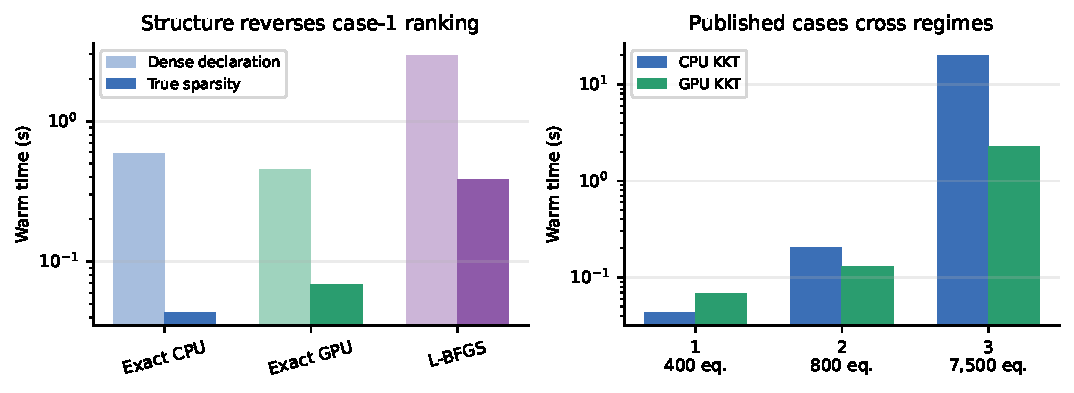
\includegraphics[width=\linewidth]{pfr_iclr.pdf}
  \caption{Published PFR-NMPC results.  \textbf{Left:} declaring the true
  derivative structure reverses the case-1 hardware ranking.  \textbf{Right:}
  preserving that structure while increasing the published horizon/state
  regime yields a CPU-to-GPU KKT crossover.}
  \label{fig:pfr}
\end{figure}

\subsection{Disclosing structure can dominate moving hardware}
\label{sec:sparsity-results}

The initial PFR port declared dense derivative coordinates.  On case~1 this
changes CPU exact from \PFRCaseOneSparseCPU\,ms to
\PFRCaseOneDenseCPU\,s---a 13.6$\times$ slowdown---and makes GPU KKT appear
preferable.  With the true 5,200/3,049 Jacobian/Hessian entries, CPU exact and
same-oracle Ipopt are essentially tied, and DLPack GPU is slower.  Thus the
hardware conclusion reverses without changing a single function value.

OMLT full space provides a formulation baseline.  At horizon 40 it expands
case~1 to 15,133 variables and 15,100 constraints and takes 21.2\,s, versus
43.3\,ms for the structure-aware gray box.  Its horizon-5 solution agrees in
objective to $4.6\times10^{-11}$.  With maintained OMLT 1.1/1.2 in the
matched software environment, reduced-space construction does not finish
within 180\,s even at horizon 5, so it has no timed entry.

Sequence behavior adds another qualification.  In the 100-step case-1 closed
loop, CPU exact obtains 100/100 common-KKT success with 29.3\,ms median,
30.4\,ms mean, and 77.5\,ms maximum.  A persistent GPU solver has a lower
24.8\,ms median, but one reuse failure triggers a rebuild, raising its mean to
62.1\,ms and maximum to 3.24\,s.  Both control trajectories stay within
$3.6\times10^{-5}$ state infinity error of the published mechanistic
trajectory.  Median-only reporting would select the less predictable
deployment and hide this tail.

The fixed replay separates initialization from persistence
(Appendix Table~\ref{tab:warm-start}).  All \PFRSequenceSuccesses/
\PFRSequenceTotal{} solves pass.  Cold CPU/GPU medians are
\PFRWarmCPUColdIter/\PFRWarmGPUColdIter{} iterations and shifted-primal medians
are \PFRWarmCPUPrimalIter/\PFRWarmGPUPrimalIter; shifted equality multipliers
change no count.  Setting $\mu_0=10^{-7}$ instead gives
\PFRWarmCPUBarrierIter/\PFRWarmGPUBarrierIter{} iterations and
\PFRWarmCPUBarrierTime/\PFRWarmGPUBarrierTime{} ms.  The setpoint change still
needs 9/10 iterations, and persistent GPU reuse still rebuilds once.  Thus
barrier initialization, not equality-dual reuse, removes the median iteration
gap; CPU KKT remains faster for this small sparse system.

\subsection{Curvature should be routed by failure and factorization cost}
\label{sec:curvature-results}

On twelve prospective public-Darcy instances and five starts at each of two
latent resolutions, compact L-BFGS reaches common KKT on
\DarcyRouteBase/\DarcyRouteTotal{} solves.  The five failures occur on three
instances.  Exact DLPack solves all 30 starts from those difficult instances.
Retrying only the five failed starts therefore reaches
\DarcyRouteTotal/\DarcyRouteTotal{} success while adding
\DarcyRouteOverhead\% to total warm time relative to L-BFGS alone.  The policy
was fixed on separate pilot instances, so this is a prospective routing result
rather than a retrospective oracle.

PFR case~3 shows why per-iteration cost is insufficient.  Compact L-BFGS avoids every
Hessian callback but needs 271 iterations and \PFRCaseThreeLBFGS\,s; 516.2\,s
is spent in linear solves.  Exact DLPack needs 11 iterations and
\PFRCaseThreeGPU\,s.  When each iteration still factorizes a 7,500-constraint
KKT system, the extra factorizations dominate the saved Hessian callbacks.

Gauss--Newton occupies a third regime.  On replayable Darcy it is faster than
exact curvature and uses fewer iterations, but explicit residual-Jacobian
formation peaks at 33.5\,GiB---the same capacity class as the exact Hessian.
It is a time approximation, not a memory-free one.  Appendix~\ref{app:curvature}
also shows that reducing L-BFGS history from 20 to 6 increases controlled
iterations from 21--35 to 64--218; history 50 yields only marginal gains over
20.  ``L-BFGS'' is itself not a parameter-free baseline.

\subsection{A surrogate KKT point is not a simulator solution}
\label{sec:validity-results}

The public Darcy experiment already signals optimization shift.  At latent 16,
the median coefficient error is 0.320 and the best representable error is
0.214; at latent 32 these values are 0.311 and 0.149.  More capacity
slightly improves recovery while nearly doubling the gap to the
parameterization floor.  Meanwhile, the optimized-to-true-coefficient FNO
residual ratio falls from 0.85 to 0.42.  Surrogate residual improves much more
than coefficient recovery.

\begin{figure}[t]
  \centering
  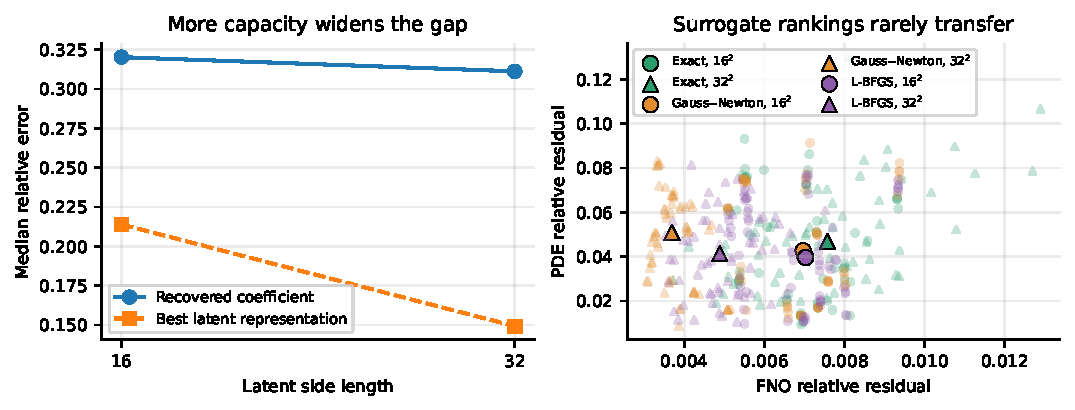
\includegraphics[width=\linewidth]{darcy_iclr.pdf}
  \caption{Optimization-aware Darcy validation.  \textbf{Left:} public-data
  coefficient error versus the best latent representation.  \textbf{Right:}
  on the independently replayable prospective split, lower FNO residual does
  not reliably imply lower sparse-PDE residual.  Markers are successful
  instance--start solves and large symbols are descriptive method medians;
  paired inference uses physical instances as the sampling unit.}
  \label{fig:darcy}
\end{figure}

Independent replay turns that signal into a direct prospective test.  Across
\ReplaySolves\ successful method/start solves on twelve disjoint instances,
\ReplayOutfitsTruth\ optimized FNO residuals are below the FNO residual at the true coefficient.
At latent 32,
Gauss--Newton is fastest (\ReplayGNTime\,s) and has the lowest median FNO
residual (\ReplayGNSurrogate\%), but its PDE residual is
\ReplayGNPDE\%.  L-BFGS is slower (\ReplayLBFGSTime\,s) and has a worse FNO
residual (\ReplayLBFGSSurrogate\%), yet its PDE residual is only
\ReplayLBFGSPDE\%.  Exact DLPack gives
\ReplayExactSurrogate\%/\ReplayExactPDE\% FNO/PDE residual.  The method
ranking agrees under surrogate and simulator in only
\ReplayAgreement/\ReplayGroups{} start-level groups.  After aggregating starts
within each physical instance, Gauss--Newton reduces FNO
residual relative to L-BFGS on all twelve instances by a median
\ReplayPairedFNOReduction\ percentage points (95\% bootstrap CI
[\ReplayPairedFNOReductionLow, \ReplayPairedFNOReductionHigh], Wilcoxon
$p=\ReplayPairedFNOPValue$).  The paired PDE change is instead
$+\ReplayPairedPDEDelta$ points with CI
[\ReplayPairedPDEDeltaLow, \ReplayPairedPDEDeltaHigh] and
$p=\ReplayPairedPDEPValue$.  Thus the evidence is a failure of surrogate gains
to transfer consistently, not proof that L-BFGS is physically superior.

An exploratory tenfold increase in Tikhonov regularization does not improve the
mismatch in this ablation: at latent 32 it raises median PDE residual from 2.37\% to 7.67\% for
L-BFGS.  Staying close to an uninformative prior is not a substitute for model
management or high-fidelity validation.

\subsection{Nonconvex timing curves require local-solution context}
\label{sec:mnist-results}

On MNIST, all methods satisfy the same raw network, slack, target, and output
bound audit, but reach different KKT points.  At 5.01M parameters, the
published start gives objective 4.644 for exact CPU, about 4.736 for exact
DLPack/L-BFGS/Ipopt-exact, and 5.625 for Ipopt limited memory.  Over five shared
starts, all \MNISTSolved/\MNISTTotal{} MadNLP solves pass; exact CPU and exact
DLPack have median objective \MNISTExactMedianObjective, while L-BFGS has
\MNISTLBFGSMedianObjective.  L-BFGS remains fastest (0.47\,s median versus
1.31\,s DLPack and 2.98\,s CPU exact), but all four perturbed starts enter
worse basins.  A speed plot without objective values would reverse the useful
interpretation.

\subsection{Memory and cold start define deployable regimes}

Exact latent-32 Darcy peaks at \DarcyExactMemory\,GiB GPU memory versus
\DarcyLBFGSMemory\,GiB for L-BFGS.  The final dense
$1024\times1024$ Hessian is only 8\,MiB: differentiated FNO intermediates, not
the returned matrix, set the capacity threshold.  PFR case~3 exact DLPack
peaks at 43.9\,GiB versus 1.14\,GiB for CPU KKT.  Conversely, its GPU
factorization supplies the decisive speedup.  Capacity and time therefore need
separate axes.

Parameter count is not a sufficient capacity proxy either.  With FNO size
matched within \FNOShapeMaxParameterMismatch\%, changing depth from one to six
layers moves the $32^2$ Hessian peak from \FNOShapeMinMemory{} to
\FNOShapeMaxMemory{} GiB and warm evaluation from \FNOShapeFastHessian{} to
\FNOShapeSlowHessian{} ms (Appendix Table~\ref{tab:topology-memory}).  Random
and trained four-layer graphs both use \FNOShapeTrainedMemory{} GiB, isolating
topology rather than learned values.

Fresh-process execution requires approximately 60--75\,s for the first JAX/cuDSS
specialization.  The case-3 DLPack cold solve takes 71.7\,s despite a
\PFRCaseThreeGPU\,s warm median.  The GPU recommendation applies to persistent
workers or repeated solves, not one-shot service calls.

\section{Discussion}
\label{sec:discussion}

\paragraph{What the regime map supports.}
The measurements define conditions, not a portable cutoff.  Transfer removal
matters only after structure and curvature determine what is moved and how many
KKT systems are solved.  PFR cases 1 and 3, latent-32 Darcy, and the fixed-size
FNO topology sweep occupy distinct regimes that parameter count or decision
dimension alone cannot identify.

A KKT certificate still belongs to the surrogate.  Independent replay links
this study to optimization shift and motivates combining failure-aware
curvature with uncertainty, model management, or periodic high-fidelity
queries.  Faster linear algebra does not replace those safeguards.

\paragraph{Threats to validity and negative results.}
Primary timings use one H100/Xeon server; shared starts and KKT audits do not
establish global optimality.  Replay Darcy is specified but not a community
benchmark, while the public split lacks historical replay.  The sequence
interface omits bound-multiplier starts, and untrained FNOs measure graph memory
rather than surrogate quality.  Appendix~\ref{app:data-audit} records the
unsupported paths, timeouts, and two invalidated errors---a transposed Darcy
target and an artificial dense-PFR GPU advantage---that made layout, sparsity,
and simulator audits decisive.

\section{Conclusion}

There is no single best curvature model or device placement for neural-
surrogate NLPs.  End-to-end GPU execution helps when repeated KKT
factorizations dominate, hurts on small sparse systems, and can exhaust memory
on neural-operator Hessians.  Parameter count, topology, barrier state, and KKT
placement describe different boundaries; a surrogate KKT point still does not
certify the simulator.

Our evidence supports a practical order: expose structure, audit common
residuals, choose curvature with failures visible, measure the device boundary,
place the KKT system, and then validate the application.  \method{} and the
benchmark suite make this regime map executable and falsifiable.


\bibliography{references_iclr}
\bibliographystyle{iclr2026/iclr2026_conference}

\paragraph{Reproducibility statement.}
Configurations, seeds, checksums, solver and failure records, derivative
audits, resource traces, and figure scripts accompany the supplement.
Appendix~\ref{app:repro} specifies the environment and exclusions.

\paragraph{Use of AI assistance.}
Language-model tools assisted with code refactoring, literature discovery, and
draft editing.  The authors are responsible for the research decisions and
verified the mathematical definitions, source translations, numerical results,
citations, and final text.

\appendix
\section{Mathematical Benchmark Definitions}
\label{app:formulations}

\subsection{Controlled oracle}

For each controlled configuration, a tanh MLP maps $x\in\R^n$ to
$N_\theta(x)\in\R^q$.  We sample a planted $x_\star$ from a fixed seed and set
$y_\star=N_\theta(x_\star)$.  The problem is
\begin{equation}
\min_{-1\leq x\leq1}
\frac{1}{2}\|N_\theta(x)-y_\star\|_2^2
+\frac{10^{-3}}{2}\|x\|_2^2
\quad\text{s.t.}\quad \|x\|_2^2\leq \tfrac14 n.
\end{equation}
All compared methods reach the same planted local solution within the common
KKT tolerance.  This family is not used as application evidence.

\subsection{Adversarial MNIST}

Let $z\in[0,1]^{784}$ be the perturbed image, $r\in\R^{10}$ the network output,
and $s^+,s^-\geq0$ $\ell_1$ slacks.  For reference image $z_0$ and target class
$t=9$, we solve
\begin{equation}
\begin{aligned}
\min_{z,r,s^+,s^-}\quad & \mathbf{1}^\top(s^++s^-)\\
\mathrm{s.t.}\quad &r-N_\theta(z)=0,\\
&z-z_0-s^++s^-=0,\\
&r_t\geq0.6,\qquad 0\leq r\leq1.
\end{aligned}
\label{eq:mnist-app}
\end{equation}
The decision dimension is 2,362.  The declared Jacobian contains the dense
$10\times784$ network input block, ten output diagonals, three entries per
slack equality, and eleven scalar probability/output entries.  Only the lower
$784\times784$ network-input Hessian block is nonlinear.

The four perturbed starts use
$\tilde z=\Pi_{[0,1]}(z_0+0.05\epsilon)$ with one fixed Gaussian draw per
start.  Network outputs are recomputed and slacks are set to the positive and
negative parts of $\tilde z-z_0$, making every network/slack equality exactly
consistent before optimization.

\subsection{Latent Darcy inversion}

Let $P_r:\R^{r^2}\rightarrow\R^{64\times64}$ be bilinear interpolation and
$G_\theta$ an FNO.  For target pressure $u_\star$, reference latent field
$a_0$, and coefficient bounds $[a_L,a_U]$, the optimized surrogate problem is
\begin{equation}
\min_{a_L\leq a\leq a_U}
\frac{1}{2|\mathcal{O}|}
\sum_{j\in\mathcal{O}}
\left(\frac{[G_\theta(P_r a)]_j-[u_\star]_j}{s_u}\right)^2
+\frac{\rho}{2r^2}\|a-a_0\|_2^2,
\label{eq:darcy-inverse-app}
\end{equation}
where $s_u$ is the target RMS and $\mathcal{O}$ contains all grid points in the
reported experiments.  The public binary-coefficient split uses $[0,1]$ and
$a_0$ equal to the training-set mean.  The replay split uses clipped
log-permeability $[-3,3]$ and $a_0=0$.

To separate optimizer error from parameterization error, we solve
\begin{equation}
e_{\mathrm{floor}}(a_\star;r)=
\min_{a_L\leq a\leq a_U}
\frac{\|P_r a-a_\star\|_2}{\|a_\star\|_2}
\end{equation}
with L-BFGS-B and strict gradient tolerances.  This projection does not use the
FNO.  The replay metric solves Equation~\ref{eq:darcy} at $P_r a$ and reports
$\|u_{\mathrm{PDE}}(P_r a)-u_\star\|_2/\|u_\star\|_2$.

\subsection{PFR-NMPC}

All PFR cases use a gray-box direct-transcription form
\begin{equation}
\begin{aligned}
\min_{x_{0:P},u_{0:M-1}}\quad &
\sum_{t=0}^{P}\|Sx_t-y^{\mathrm{sp}}\|_{Q}^{2}
+\sum_{t=0}^{M-1}\|u_t-u_{t-1}\|_{R}^{2}\\
\mathrm{s.t.}\quad &x_{t+1}=N_\theta(x_t,u_{\min(t,M-1)}),
\quad t=0,\ldots,P-1,\\
&x_0=x_{\mathrm{meas}},\qquad \ell_x\leq x_t\leq u_x,
\quad \ell_u\leq u_t\leq u_u.
\end{aligned}
\label{eq:pfr-app}
\end{equation}
Selection $S$, targets, scales, bounds, and horizons are read from the released
case files.  Case~1 has $P=40,M=10$ and a tanh MLP.  Case~2 has $P=40,M=10$
and a convolutional surrogate over two 10-point state fields.  Case~3 has
$P=30,M=10$ and a convolutional surrogate over five 50-point fields.

\section{Interface and Numerical Correctness Audits}
\label{app:audits}

\subsection{DLPack ownership and synchronization}

The Julia buffer owner outlives every imported JAX view.  A custom DLPack
capsule transfers a view, not ownership of the CUDA allocation.  Separate tests
verify (i) identical device pointers after import, (ii) Julia-to-JAX and
JAX-to-Julia mutation visibility, (iii) dtype and shape preservation, and
(iv) synchronization before timing boundaries.  Derivative output arrays are
not aliased into MadNLP: JAX computes them in its allocator and a device copy
places coordinates in solver-owned buffers.  This avoids lifetime ambiguity
while eliminating host staging.

\subsection{Array-layout invariant}

NumPy/JAX flatten a two-dimensional target in row-major order, whereas Julia's
\texttt{vec} uses column-major order.  Every Julia--Python field conversion
therefore applies the explicit row-major invariant
\texttt{vec(permutedims(field))}.  For normalized least squares with negligible
regularization, $\sqrt{2f}$ must agree with the independently computed relative
field residual.  A regression test enforces this relation.

\subsection{Parity and directional derivatives}

\begin{table}[ht]
\centering
\caption{Representative float64 translation and derivative gates.  Errors are
relative $\ell_2$ discrepancies; finite differences are central.}
\label{tab:audits}
\small
\begin{tabular}{lrrrr}
\toprule
Oracle & Torch/JAX & $Df[v]$ & $Jv$ & $\nabla^2\mathcal{L}v$\\
\midrule
PDEBench FNO & $1.5\times10^{-7}$ & $1.8\times10^{-12}$ & $7.7\times10^{-13}$ & $2.6\times10^{-12}$\\
Replay FNO & $2.4\times10^{-16}$ & --- & --- & $6.0\times10^{-11}$\textsuperscript{a}\\
PFR case 1 & $9.3\times10^{-16}$ & $3.7\times10^{-11}$ & $3.4\times10^{-10}$ & $4.6\times10^{-11}$\\
PFR case 2 & $3.1\times10^{-16}$ & $1.6\times10^{-7}$ & $3.6\times10^{-9}$ & $5.9\times10^{-8}$\\
PFR case 3 & $1.4\times10^{-16}$ & $2.7\times10^{-10}$ & $5.2\times10^{-9}$ & $1.1\times10^{-10}$\\
MNIST & $1.8\times10^{-15}$ & --- & $<7\times10^{-8}$ & $<7\times10^{-8}$\\
\bottomrule
\end{tabular}
\parbox{0.94\linewidth}{\footnotesize \textsuperscript{a}Independent
Gauss--Newton directional quadratic-form check.}
\end{table}

Float32 parity is also tested and is below $7.4\times10^{-7}$ across retained
models.  High-precision JAX matrix multiplication is part of provenance:
disabling it caused a reproducible $\sim5\times10^{-4}$ discrepancy for the
PDEBench FNO.

\section{Extended Curvature Results}
\label{app:curvature}

\subsection{Controlled L-BFGS history sensitivity}

\begin{figure}[ht]
  \centering
  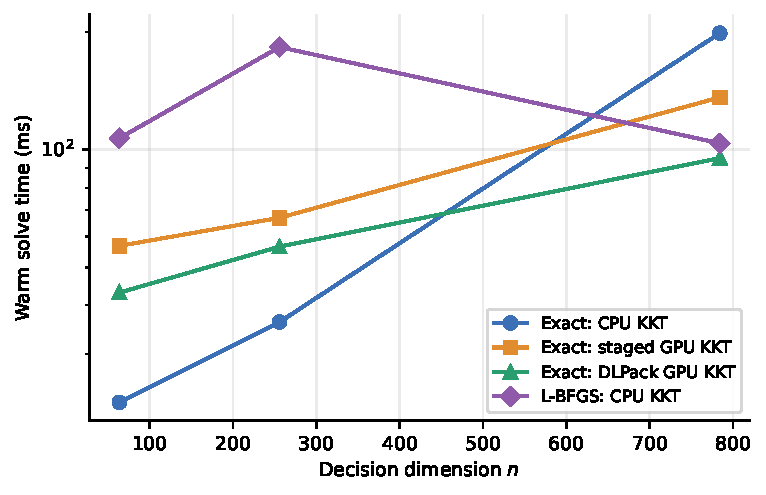
\includegraphics[width=0.72\linewidth]{controlled_regime.pdf}
  \caption{Controlled warm solves at a common KKT point.  CPU KKT wins for
  small decision spaces; at $n=784$, DLPack GPU KKT wins within exact
  curvature, while L-BFGS changes the ranking again.}
  \label{fig:controlled-app}
\end{figure}

\begin{table}[ht]
\centering
\caption{Compact L-BFGS history sensitivity on the controlled family.  Times
are medians of ten warm runs except history 20, for which the available
measurement has three warm repetitions.}
\label{tab:history}
\small
\begin{tabular}{rrrrrrrr}
\toprule
& \multicolumn{2}{c}{History 6} & \multicolumn{2}{c}{History 20} & \multicolumn{2}{c}{History 50}\\
$n$ & time (s) & iter & time (s) & iter & time (s) & iter\\
\midrule
64  & 1.044 & 218 & 0.107 & 29 & \textbf{0.080} & 25\\
256 & 0.831 & 160 & 0.183 & 35 & \textbf{0.166} & 31\\
784 & 0.401 & 64  & \textbf{0.104} & 21 & 0.107 & 21\\
\bottomrule
\end{tabular}
\end{table}

History 6 reduces stored pairs but loses too much curvature information.  A
history of 50 is slightly better for the two small cases and statistically
indistinguishable in practical terms at $n=784$.  We retain history 20 across
applications as a fixed compact default rather than tuning per instance.

\subsection{Public Darcy placement and curvature}

\begin{table}[ht]
\centering
\caption{Public-Darcy median-instance warm time / iterations.}
\label{tab:darcy-paths}
\small
\setlength{\tabcolsep}{3pt}
\begin{tabular}{rcccc}
\toprule
Latent & Exact CPU & Host-staged GPU & DLPack GPU & L-BFGS CPU\\
\midrule
$8^2$  & 0.125 / 12 & 0.164 / 12 & 0.158 / 12 & \textbf{0.105} / 33\\
$16^2$ & 0.605 / 18 & 0.648 / 18 & 0.636 / 18 & \textbf{0.216} / 38\\
$32^2$ & 4.716 / 22 & 2.898 / 22 & 2.752 / 22 & \textbf{0.961} / 46\\
\bottomrule
\end{tabular}
\end{table}

At $32^2$, DLPack is 1.7$\times$ faster than CPU KKT within exact curvature,
and 5\% faster than host staging.  L-BFGS is another 2.9$\times$ faster than
exact DLPack on the successful median-instance start.  The prospective failure
audit in the main text is what prevents promoting that single-start result to
a universal recommendation.

\subsection{Prospective replay and regularization intervention}

\begin{table}[ht]
\centering
\caption{Prospective replay-Darcy medians over twelve disjoint instances and
five starts (60 attempts per row); all 360 solves pass common KKT.}
\label{tab:replay-prospective}
\small
\setlength{\tabcolsep}{3pt}
% Auto-generated prospective replay table.
\begin{tabular}{llrrrr}
\toprule
Latent & Curvature & time (s) & FNO res. & PDE res. & coeff. err.\\
\midrule
$16^2$ & Exact DLPack & 0.492 & 0.70\% & 4.08\% & 21.5\%\\
$16^2$ & Gauss--Newton & 0.238 & 0.70\% & 4.26\% & 21.4\%\\
$16^2$ & L-BFGS CPU & 0.879 & 0.70\% & 3.96\% & 21.3\%\\
\midrule
$32^2$ & Exact DLPack & 1.949 & 0.76\% & 4.68\% & 43.8\%\\
$32^2$ & Gauss--Newton & 0.714 & 0.37\% & 5.09\% & 22.3\%\\
$32^2$ & L-BFGS CPU & 1.428 & 0.49\% & 4.13\% & 28.8\%\\
\bottomrule
\end{tabular}

\end{table}

\begin{table}[ht]
\centering
\caption{Latent-32 paired effects with one median per physical instance.
Negative favors Gauss--Newton.  The bootstrap resamples twelve instances.}
\label{tab:replay-paired}
\small
% Auto-generated paired effects; unit is one physical instance.
\begin{tabular}{lrrr}
\toprule
Metric (GN $-$ L-BFGS) & median (pp) & bootstrap 95\% CI & Wilcoxon $p$\\
\midrule
FNO residual & -0.095 & [-0.133, -0.065] & 0.00049\\
PDE residual & 1.20 & [-1.10, 2.96] & 0.266\\
\bottomrule
\end{tabular}

\end{table}

Increasing $\rho$ in Equation~\ref{eq:darcy-inverse-app} from $10^{-4}$ to
$10^{-3}$ is an exploratory intervention on the three development instances.
For L-BFGS at latent 32 it
raises median FNO residual from 0.49\% to 1.02\%, PDE residual from 2.37\% to
7.67\%, and coefficient error from 29.9\% to 42.9\%.  A generic distance-to-
mean penalty does not encode the Gaussian-field correlation structure and is
not retained as a method.

\vfill
\section{Extended Solver and Resource Tables}
\label{app:extended}

\begin{table}[ht]
\centering
\caption{Evidence-backed decision order.  Each recommendation requires the
preceding audit; none follows from network parameter count alone.}
\label{tab:decisions}
\small
\setlength{\tabcolsep}{3.3pt}
\begin{tabular}{p{0.21\linewidth}p{0.30\linewidth}p{0.37\linewidth}}
\toprule
Observed regime & Default action & Required qualification\\
\midrule
Sparse, small KKT & CPU exact & Declare true $J/H$ structure first\\
Large $p$, modest $n,m$ & GPU AD, CPU KKT & Measure transfer and callback share\\
Large $n$, costly Hessian AD & L-BFGS first & Exact same-start fallback on KKT failure\\
Large repeated KKT & DLPack + GPU KKT & Amortize cold start; report memory and tails\\
Learned physical surrogate & Independent replay & Do not rank methods by surrogate loss alone\\
\bottomrule
\end{tabular}
\end{table}

\subsection{PFR case 1 paths}

\begin{table}[ht]
\centering
\caption{PFR case-1 first-step results after structure correction.}
\small
\begin{tabular}{lrrl}
\toprule
Method & warm median & success & note\\
\midrule
MadNLP exact, CPU KKT & 43.3 ms & 5/5 & 5,200 Jacobian entries\\
cyipopt exact & 43.9 ms & 3/3 & same JAX oracle\\
MadNLP exact, DLPack GPU & 68.9 ms & 5/5 & device-native boundary\\
MadNLP exact, staged GPU & 89.1 ms & 5/5 & host transfer control\\
MadNLP compact L-BFGS & 385 ms & 5/5 & 61 iterations\\
Ipopt limited memory & 880 ms & 3/3 & raw audit passes\\
OMLT full space + Ipopt & 21.2 s & 3/3 & horizon 40\\
\bottomrule
\end{tabular}
\end{table}

\subsection{MNIST scale and multi-start}

\begin{table}[H]
\centering
\caption{MNIST published-start warm times in seconds.  Bold is fastest, not
necessarily the best local objective.}
\small
\setlength{\tabcolsep}{3pt}
\begin{tabular}{rccccc}
\toprule
$p$ & Exact CPU & Exact DLPack & L-BFGS CPU & Ipopt exact & Ipopt LM\\
\midrule
0.168M & 0.895 & \textbf{0.401} & 0.403 & 1.739 & 1.535\\
1.46M  & 2.968 & 0.567 & \textbf{0.231} & 3.412 & 1.651\\
5.01M  & 1.511 & 1.327 & \textbf{0.275} & 4.555 & 2.447\\
\bottomrule
\end{tabular}
\end{table}

For the five-start 5.01M study, exact CPU has median/range objective
4.736/(4.644--5.590), exact DLPack 4.736/(4.736--4.999), and L-BFGS
5.590/(4.736--5.625).  All five starts pass for each method.

\subsection{Whole-process peak memory}

\begin{table}[H]
\centering
\caption{Fresh-process memory peaks with JAX preallocation disabled.}
\label{tab:memory}
\small
\begin{tabular}{llrr}
\toprule
Problem & Method & host GiB & GPU GiB\\
\midrule
PFR case 1 & exact CPU KKT & 3.72 & 0.86\\
PFR case 1 & exact DLPack & 4.17 & 1.08\\
PFR case 3 & exact CPU KKT & 4.47 & 1.14\\
PFR case 3 & exact DLPack & 6.15 & 43.90\\
PFR case 3 & L-BFGS CPU KKT & 4.15 & 1.14\\
MNIST 5.01M & exact DLPack & 4.91 & 2.77\\
MNIST 5.01M & L-BFGS CPU KKT & 8.27 & 1.05\\
Darcy $32^2$ & exact DLPack & 5.76 & 33.54\\
Darcy $32^2$ & Gauss--Newton & 5.75 & 33.51\\
Darcy $32^2$ & L-BFGS CPU KKT & 3.96 & 0.99\\
\bottomrule
\end{tabular}
\end{table}

JAX device-memory preallocation is disabled for every entry in
Table~\ref{tab:memory}; otherwise allocator reservation, rather than peak
algorithmic demand, would dominate the measurement.

\subsection{Sequence initialization and parameter-matched topology}

Every sequence policy replays the same published states and exogenous controls.
The cold policy rolls the network forward from the current state with a fixed
control initializer.  The primal policy shifts the preceding state/control
trajectory by one step; primal--dual also shifts equality multipliers.  The
barrier variants set $\mu_0=10^{-7}$.  MadNLP does not expose initial bound
multipliers, so this is not a complete primal--dual--barrier warm start.
Steady summaries omit the first solve and the setpoint discontinuity at step 51.
All variants pass the shared $10^{-6}$ KKT audit.  Barrier-aware starts finish
closer to that threshold (maximum KKT error $9.8\times10^{-7}$) and deviate by
at most $\PFRWarmBarrierControlError$ from the published control; Table~\ref{tab:warm-start}
therefore reports iteration savings together with success rather than treating
the lower count as a stronger solution certificate.
At $10^{-8}$, the CPU median changes from \PFRStrictCPUPrimalIter{} to
\PFRStrictCPUBarrierIter{} iterations, while the GPU median remains
\PFRStrictGPUPrimalIter{} with or without the smaller barrier
(Table~\ref{tab:warm-start-tolerance}).  The cross-device median gap still
closes, but the stricter test does not support a universal GPU iteration gain
from lowering $\mu_0$.

The topology sweep fixes 12 Fourier modes, float64 arithmetic, $64^2$ full
resolution, $32^2$ latent resolution, and dense exact-Hessian construction.
Depth/width pairs $(1,64),(2,45),(3,37),(4,32),(6,26)$ differ by at most
\FNOShapeMaxParameterMismatch\% in parameter count.  Seeded untrained networks
instantiate the static graphs only; the four-layer trained/random control
separates graph shape from weight values.  No predictive or optimization claim
uses the untrained models.

% Generated by experiments/analysis/analyze_sequence_and_topology.py
\begin{table}[t]
\centering
\caption{PFR case-1 initialization ablation on one fixed 100-step replay. Steady statistics exclude the first solve and the setpoint change at step 51; iterations are median (95th percentile). Every entry uses the same exact derivatives and passes the common KKT audit.}
\label{tab:warm-start}
\small
\begin{tabular}{llrrrr}
\toprule
KKT & initialization & success & iterations & median ms & step-51 iter.\\
\midrule
CPU & cold rollout & 100/100 & 10 (10) & 41.9 & 9\\
CPU & shifted primal & 100/100 & 6 (6) & 28.4 & 9\\
CPU & primal + $\mu_0=10^{-7}$ & 100/100 & 3 (4) & 17.1 & 9\\
CPU & shifted primal--dual & 100/100 & 6 (6) & 27.6 & 9\\
CPU & primal--dual + $\mu_0=10^{-7}$ & 100/100 & 3 (4) & 16.0 & 9\\
GPU & cold rollout & 100/100 & 10 (11) & 67.5 & 10\\
GPU & shifted primal & 100/100 & 4 (8) & 37.9 & 11\\
GPU & primal + $\mu_0=10^{-7}$ & 100/100 & 3 (5) & 32.9 & 10\\
GPU & shifted primal--dual & 100/100 & 4 (8) & 37.8 & 11\\
GPU & primal--dual + $\mu_0=10^{-7}$ & 100/100 & 3 (5) & 32.1 & 10\\
GPU reuse & persistent solver & 100/100 & 4 (8) & 22.3 & 12\\
\bottomrule
\end{tabular}
\end{table}

\begin{table}[t]
\centering
\caption{Exact-Hessian memory under parameter-matched FNO topology changes. All networks use 12 Fourier modes and $32^2$ latent variables; parameter counts differ by at most 1.1\%. Random checkpoints are used only to instantiate static AD graphs; the two four-layer rows verify that trained and random weights yield the same allocation.}
\label{tab:topology-memory}
\small
\begin{tabular}{rrrrrr}
\toprule
layers & width & parameters & GPU GiB & warm Hessian s & trained\\
\midrule
1 & 64 & 1.193M & 32.72 & 0.065 & no\\
2 & 45 & 1.177M & 32.74 & 0.088 & no\\
3 & 37 & 1.192M & 34.74 & 0.105 & no\\
4 & 32 & 1.188M & 32.77 & 0.110 & yes\\
4 & 32 & 1.188M & 32.77 & 0.110 & no\\
6 & 26 & 1.176M & 37.25 & 0.132 & no\\
\bottomrule
\end{tabular}
\end{table}

\begin{table}[t]
\centering
\caption{Tolerance sensitivity on the same replay. Steady iterations are median (95th percentile); all solves satisfy $10^{-8}$.}
\label{tab:warm-start-tolerance}
\small
\begin{tabular}{llrrr}
\toprule
KKT & initialization & success & iterations & median ms\\
\midrule
CPU & shifted primal & 100/100 & 6 (7) & 28.7\\
CPU & primal + $\mu_0=10^{-7}$ & 100/100 & 4 (5) & 21.0\\
GPU & shifted primal & 100/100 & 4 (6) & 39.4\\
GPU & primal + $\mu_0=10^{-7}$ & 100/100 & 4 (8) & 39.5\\
\bottomrule
\end{tabular}
\end{table}


The topology table isolates one Hessian evaluation rather than a complete NLP
solve.  Its trained four-layer peak of \FNOShapeTrainedMemory{} GiB is therefore
slightly below the \DarcyExactMemory-GiB whole-process peak in
Table~\ref{tab:memory}.  Replacing the trained weights by seeded random weights
leaves the peak unchanged at \FNOShapeRandomMemory{} GiB, as expected for a
static compiled graph.  A process-scoped allocation check on a 96-GB
Blackwell GPU reproduces every topology peak within
\FNOShapeCrossHardwareDelta{} GiB; its timings are excluded because that device
was not under the primary timing protocol.

\section{Benchmark and Data Audit Trail}
\label{app:data-audit}

\paragraph{Excluded synthetic variants.}
We exclude an inversion variant in which the target was generated by the same
FNO being inverted and initialization used the hidden coefficient; this is an
inverse crime and does not test generalization.  We also exclude a synthetic
Pareto task whose hypervolume reference depended on the returned points.  Both
remain software-level verification cases, not application benchmarks.

\paragraph{PDEBench audit.}
The official beta-1 file and FNO checkpoint pass checksum, forward-parity, and
derivative gates.  Across its 1,000 held-out samples, FNO pressure-error
quartiles are 14.8\%, 17.3\%, and 20.9\%.  Source inspection shows that the
file named DarcyFlow evolves a random initial field under variable-coefficient
diffusion while releasing only the coefficient/terminal label pair.  The
unobserved random initial condition prevents deterministic replay.  We retain
the model for AD, transfer, layout, and memory interoperability tests, not inverse-design
claims \citep{takamoto2022pdebench}.

\paragraph{Public elliptic Darcy.}
The maintained NeuralOperator loader references a public 5,000/1,000
$64\times64$ split.  Its binary coefficient and solution are deterministic,
but the archive omits the coefficient mapping and fine-grid/downsampling
metadata of the historical MATLAB solver.  Trying documented $4/12$ and
$0.1/1$ mappings does not meet a predeclared replay tolerance.  We therefore
report coefficient truth and latent representability, not a fitted ``physics''
residual.

\paragraph{Registered replay split.}
The fallback split stores continuous zero-mean Gaussian-random-field
log-permeability clipped to $[-3,3]$, with train/test seeds 20260823/20260824.
Equation~\ref{eq:darcy} is solved in float64 before storage.  The manifest
contains SHA-256 checksums of both tensors and the selected FNO.  It is labeled
a fully specified standard-equation split, not a public community benchmark.

\section{Reproducibility Details}
\label{app:repro}

\paragraph{Hardware and software.}
Experiments use a single server with one NVIDIA H100 SXM 80GB GPU, two Intel
Xeon Platinum 8562Y+ sockets (64 physical cores, 128 hardware threads), and
approximately 1\,TiB host memory.  Primary versions are Julia 1.12.7, MadNLP
0.10, MadNLPGPU 0.10, CUDSS.jl 0.8, Python 3.11, JAX 0.10, and PyTorch 2.11
with CUDA 12.8.  CPU affinity is fixed and Julia/BLAS/OpenMP use one thread for
latency measurements; complete environment locks are supplied.

\paragraph{Reproduction material.}
The supplement contains configurations, seeds, data/checkpoint checksums, raw
records, resource traces, derivative/parity audits, and all table/figure
scripts.  Timed records include solver options, cold/warm designation,
termination and residuals, and device placement; integration tests cover
staged and DLPack paths.

\paragraph{Failure and exclusion policy.}
All unsuccessful attempts contribute to success denominators.  Correctness-
based exclusions (target layout, unsafe reuse, or allocator preallocation) are
documented; no run is excluded by runtime or solution quality.  Public data and
checkpoints are identified by checksum.


\end{document}
